\chapter{Estadísticas y Métricas de Rendimiento}

Se detallan las métricas y estadísticas de rendimiento recopiladas durante las ejecuciones de prueba del generador de 
imágenes tipo \textit{cartoon}. Se describen los entornos de prueba, las configuraciones experimentales analizadas y se 
presentan los gráficos resultantes para visualizar el comportamiento de las distintas implementaciones paralelas.

\section{Métricas de Rendimiento}

Para evaluar y comparar cuantitativamente el desempeño de las implementaciones paralelas en relación con la versión 
secuencial de referencia, se utilizaron las siguientes métricas estándar:

\begin{itemize}
    \item \textbf{Tiempo de ejecución ($T_p$):} El tiempo total medido en segundos empleado en el procesamiento 
    de la imagen. Para garantizar la precisión de la medición del algoritmo en sí, este tiempo excluye las operaciones 
    de entrada/salida (I/O) en disco (carga de la imagen original y guardado del archivo final procesado).
    
    \item \textbf{Speedup o Aceleración ($S_p$):} Representa la ganancia de velocidad obtenida al utilizar recursos 
    paralelos en comparación con el algoritmo secuencial. Se define mediante la fórmula:
    \[S_p = \frac{T_1}{T_p}\]
    Donde $T_1$ es el tiempo de ejecución secuencial y $T_p$ es el tiempo de ejecución con la versión paralela 
    utilizando $p$ unidades de recursos (threads o procesos). Un speedup ideal sería uno super lineal.
    
\end{itemize}

\section{Configuraciones Experimentales}

Las pruebas de rendimiento se llevaron a cabo variando múltiples parámetros del algoritmo y del entorno para analizar 
el comportamiento bajo distintas intensidades de cómputo y comunicación:

\begin{enumerate}
    \item \textbf{Resolución de las Imágenes:} Se utilizaron tres resoluciones con distinta cantidad de carga de trabajo:
    \begin{itemize}
        \item \textbf{Baja ($800 \times 800$ píxeles):} Carga de trabajo ligera ($640$ mil píxeles).
        \item \textbf{Media ($2000 \times 2000$ píxeles):} Carga de trabajo moderada ($4$ millones de píxeles).
        \item \textbf{Alta ($5000 \times 5000$ píxeles):} Carga de trabajo pesada ($25$ millones de píxeles).
    \end{itemize}
    
    \item \textbf{Intensidad del Filtro de Convolución (Borroneado):}
    \begin{itemize}
        \item \textbf{Filtro 3$\times$3 (Radio 1):} Requiere menor cantidad de operaciones por píxel.
        \item \textbf{Filtro 5$\times$5 (Radio 2):} Requiere mayor cantidad de operaciones de vecindad por píxel.
    \end{itemize}
    
    \item \textbf{Rangos de Posterizado:}
    \begin{itemize}
        \item \textbf{3 Rangos (Parámetro 1):} Pocos intervalos de discretización de color.
        \item \textbf{9 Rangos (Parámetro 2):} Mayor granularidad en el cálculo del color final.
    \end{itemize}

    \item \textbf{Recursos y Paradigmas Asignados:}
    \begin{itemize}
        \item \textbf{Secuencial:} Ejecución base con un solo thread/proceso ($1$ recurso).
        \item \textbf{Graphics Processing Unit (GPU):} evaluado en configuraciones de bloques con \textit{Tiles} de $8\times8$, $16\times16$, $24\times24$ y $32\times32$, correspondientes a $64$, $256$, $576$ y $1024$ threads por bloque.
    \end{itemize}
\end{enumerate}

\section{Visualizaciones de Desempeño}

A continuación, se presentan el gráfico generado para representar de manera sintética el comportamiento del sistema.


\subsection*{Heatmap de Speedup por Escenario}
El heatmap permite cruzar todas las ejecuciones (combinaciones de resolución, filtro y posterización en el eje X) con todas las configuraciones de 
recursos (eje Y), mapeando el speedup absoluto en una escala de color.

\begin{figure}[H]
    \centering
    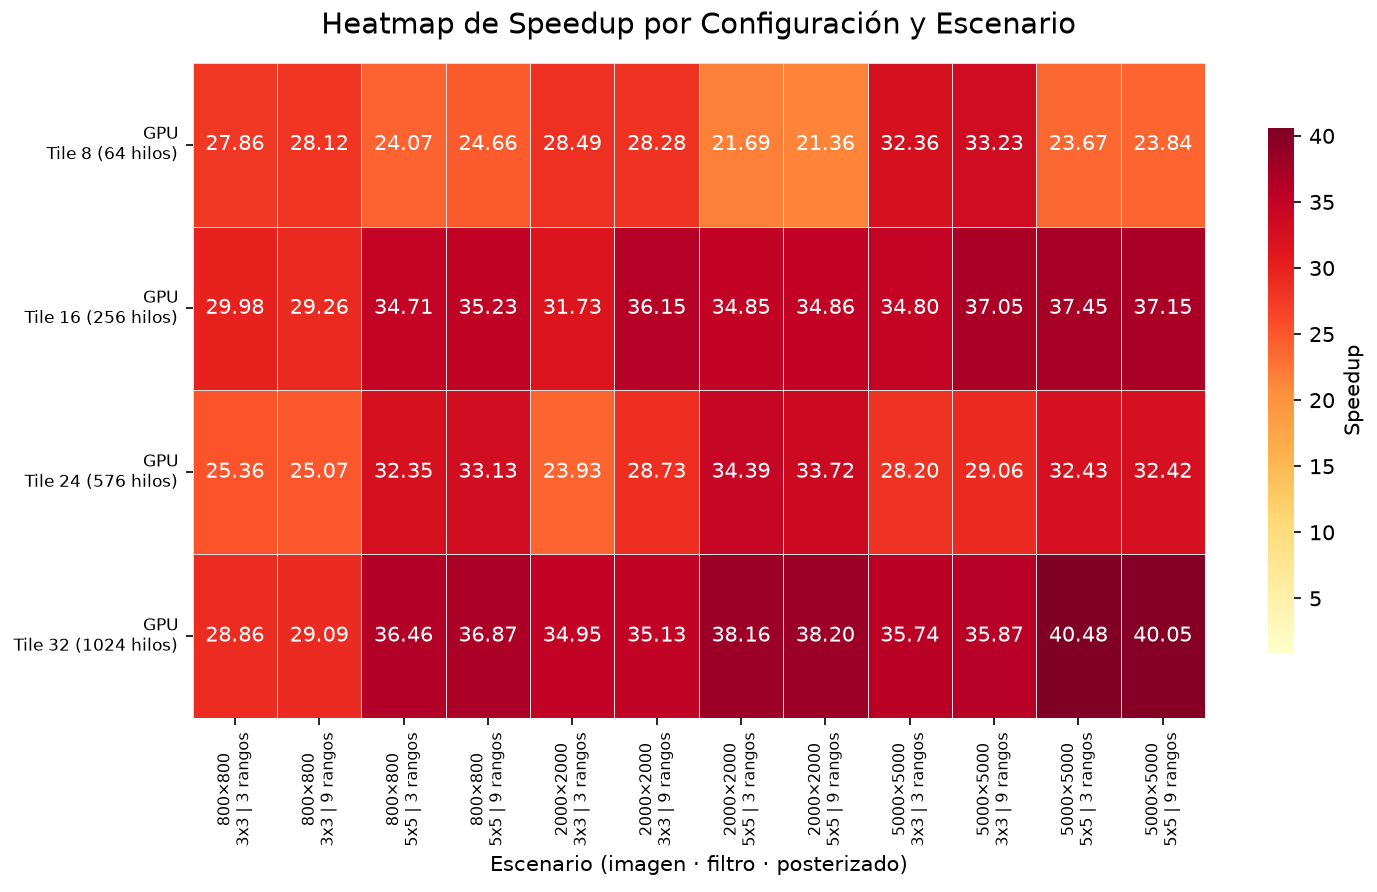
\includegraphics[width=0.95\textwidth]{resources/benchmark_gpu-heatmap_speedup.png}
    \caption{Heatmap de Speedup detallado por escenario y configuración.}
    \label{fig:heatmap}
\end{figure}

\subsection*{Análisis de Escalabilidad por Tamaño de Imagen}
La gráfica de escalabilidad permite analizar la evolución del \textit{speedup} promedio de las distintas configuraciones de GPU (según el tamaño de \textit({Tile}) y números de threads) a medida que incrementa la resulución de la imagen y la carga de cómputo asociada (desde $800\times800$ hasta $5000\times5000$ píxeles).

\begin{figure}[H]
    \centering
    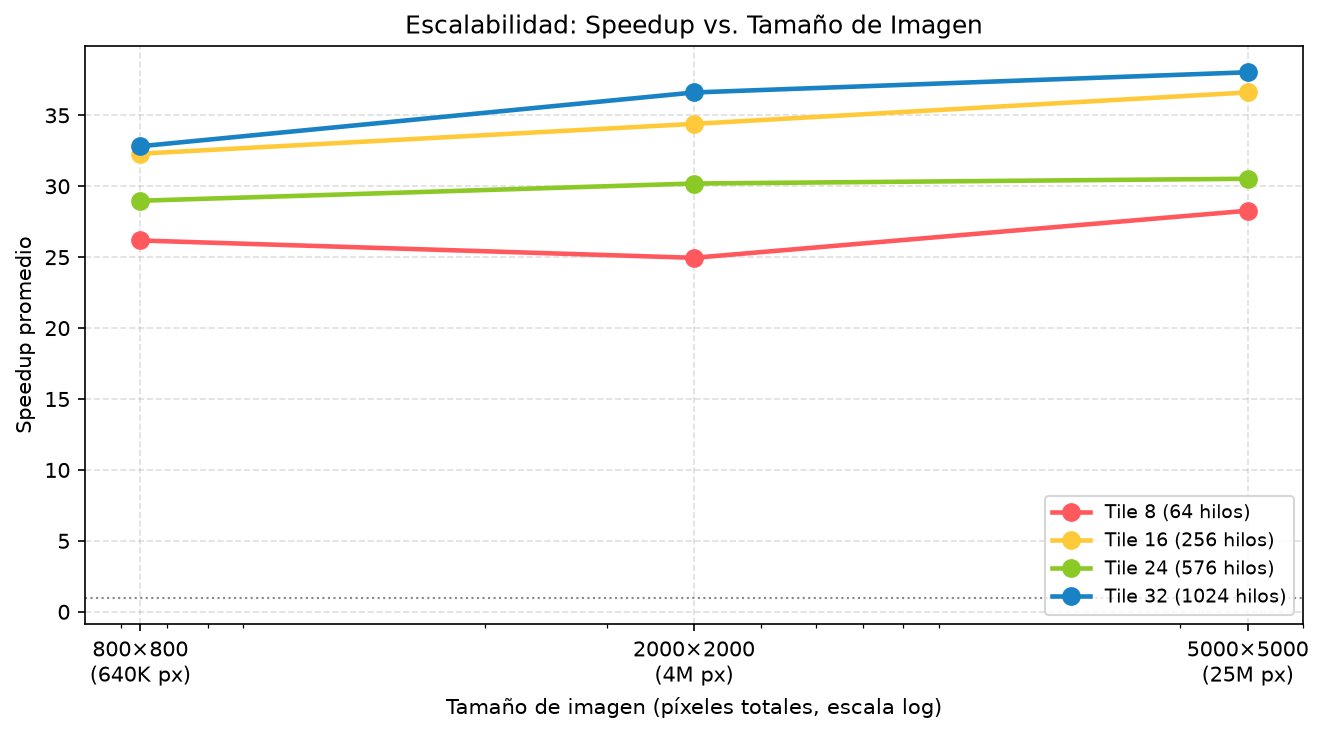
\includegraphics[width=0.95\textwidth]{resources/benchmark_gpu-escalabilidad.png}
    \caption{Evolución del speedup de la GPU frente al tamaño de la imagen.}
    \label{fig:escalabilidad}
\end{figure}


\bigbreak
\noindent \textit{Nota: Las tablas numéricas de datos crudos obtenidas de cada ejecución se encuentran adjuntas en 
los Anexos \ref{appendix:local}.}
